\documentclass{standalone}
%-----------------------------------------------------------------------------%
%%% Color %%%
\usepackage{xcolor}
\definecolor{myred}{RGB}{229,0,0}
\definecolor{myblue}{RGB}{0,98,144}
\definecolor{myyellow}{RGB}{246,182,50}
\definecolor{mygreen}{RGB}{75,108,89}
\newcommand{\red}[1]{\textcolor{myred}{#1}}
\newcommand{\blue}[1]{\textcolor{myblue}{#1}}
\newcommand{\yellow}[1]{\textcolor{myyellow}{#1}}
%-----------------------------------------------------------------------------%
\usepackage{customdice}
%-----------------------------------------------------------------------------%
%%% TikZ %%%
\usepackage{tikz}
% \usetikzlibrary{calc}
% \usetikzlibrary{positioning}
% \usetikzlibrary{patterns}
% \usetikzlibrary{fit}
\usetikzlibrary{angles,quotes}
% \usetikzlibrary{intersections}
% \usetikzlibrary{decorations.markings}
%-----------------------------------------------------------------------------%

\begin{document}

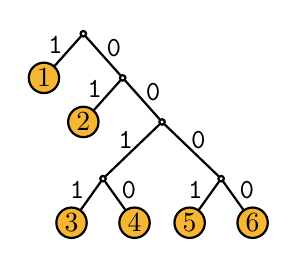
\begin{tikzpicture}[thick,line cap=round,yscale=0.8]
	\tikzstyle{bai}=[solid,circle,draw,inner sep=.07em,fill=white];
	\tikzstyle{hei}=[solid,circle,draw,inner sep=.07em,fill];
	\tikzstyle{endnode}=[solid,circle,draw,inner sep=.1em,fill=myyellow];
	\tikzstyle{encode}=[pos=0.3]
	\tikzstyle{level 1}=[level distance=0.7cm, sibling distance=1cm];
	\tikzstyle{level 2}=[level distance=0.7cm, sibling distance=1cm];
	\tikzstyle{level 3}=[level distance=0.9cm, sibling distance=1.5cm];
	\tikzstyle{level 4}=[level distance=0.7cm, sibling distance=0.8cm]; 
	\node[bai]{}
		child {
			node[endnode] {$\dice{1}$}
			edge from parent node[encode,left] {$\mathtt{1}$}
		}
		child {
			node[bai] {}
			child {
				node[endnode] {$\dice{2}$} 
				edge from parent node[encode,left]  {$\mathtt{1}$}
			}
			child {
				node[bai] {}
				child {
					node[bai] {}
					child {
						node[endnode] {$\dice{3}$}
						edge from parent node[encode,left]  {$\mathtt{1}$}
					}
					child {
						node[endnode] {$\dice{4}$}
						edge from parent node[encode,right]  {$\mathtt{0}$}
					}
					edge from parent node[encode,left]  {$\mathtt{1}$}
				}
				child {
					node[bai] {}
					child {
						node[endnode] {$\dice{5}$}
						edge from parent node[encode,left]  {$\mathtt{1}$}
					}
					child {
						node[endnode] {$\dice{6}$}
						edge from parent node[encode,right]  {$\mathtt{0}$}
					}
					edge from parent node[encode,right]  {$\mathtt{0}$}
				}
				edge from parent node[encode,right] {$\mathtt{0}$}
			}
			edge from parent node[encode,right] {$\mathtt{0}$}
		};
\end{tikzpicture}

\end{document}
